\section{Web UI Investigation Tool}

The web application is designed as a single page web-application, such that changes in the URL represent the application rendering a different view dynamically, rather than making a request for a new web-page. 

\subsection{Technology Choices}
\subsubsection{Angular 6 \& TypeScript}
Angular 6 provides excellent tooling for scaffolding out a wire-frame for the application and scaffolding out individual components. This is achievable using the \texttt{@angular-cli} tool where a command as simple as \texttt{ng new my-app; cd my-app; ng serve} will have a wire-frame web application up and running. This was a lucrative feature of Angular for this project, since it would help expedite the web-application setup process and facilitate more time to be spent on developing features.
\\\\
Angular 6 applications are written in TypeScript; a statically typed super-set of JavaScript. Using a statically-typed language is a personal preference of mine, where possible, in order to allow for some compile time type-checking and easier refactoring. 
\\\\
Angular comes with RxJS, an asynchronous programming library. This provides a new approach to asynchronous requests than simple Promises in JavaScript, which can only be subscribed to once. RxJS provide Observables which can be subscribed and listened to indefinitely and provide any number of date updates. This is particularly useful for my application since every interaction the user makes with the graph will initiate an asynchronous request to fetch the data to render further nodes/information. These requests may be made concurrently too, so having a single Observable to listen for all new 'block' or 'transaction' information, for instance, would greatly simplify my implementation. 
\\\\
\textbf{Alternatives to Angular}: React is another solution to building single-page web-applications that is popular in the industry. However, React is a library whereas Angular is a fully-fledged MVC framework providing far more 'out-the-box' functionality. React only provides the 'V' (the view) and will require several other libraries to fill in the model and controller components of MVC. Due to my familiarity with Angular, and comparatively unfamiliar with React, there would potentially be a steep learning curve adopting React for this project, in addition to the several libraries I may require to integrate with. Angular would allow me to build and iterate fast since much of the basic functionality is provided by Angular.

\subsubsection{D3}
D3.js is a JavaScript library that can be used for generating SVG visualisations in the DOM. D3 has no direct connection to Neo4J, unlike some other tools. The data will therefore be retrieved using my own database API and will therefore involve further steps to fetch the data to render; however, this is advantageous as it will provide the flexibility to customise the API implementation to orchestrate responses by making customised queries or communicating with several data stores.
\\\\
\textbf{Alternatives to D3}: There exist some visualisation tools that have embedded connections to Neo4J. I initially considered these tools as a possible simplification of the visualisation element of the web application; however, these tools such as Neovis.js and Popoto.js seem too restrictive in that their data format must align with the data format in Neo4J. They appear to be very suitable for visually mirroring the data in Neo4J, but I believe for this project, with the scope for many visual features with data persisted in locations other than Neo4J, this will prove to be too constraining. As for other JavaScript libraries similar to D3 with high customisability, I chose D3 due to the abundance of documentation, community support and example projects that D3 has. 

\subsection{Implementation}
\begin{sidewaysfigure}[h!]
  \centering
  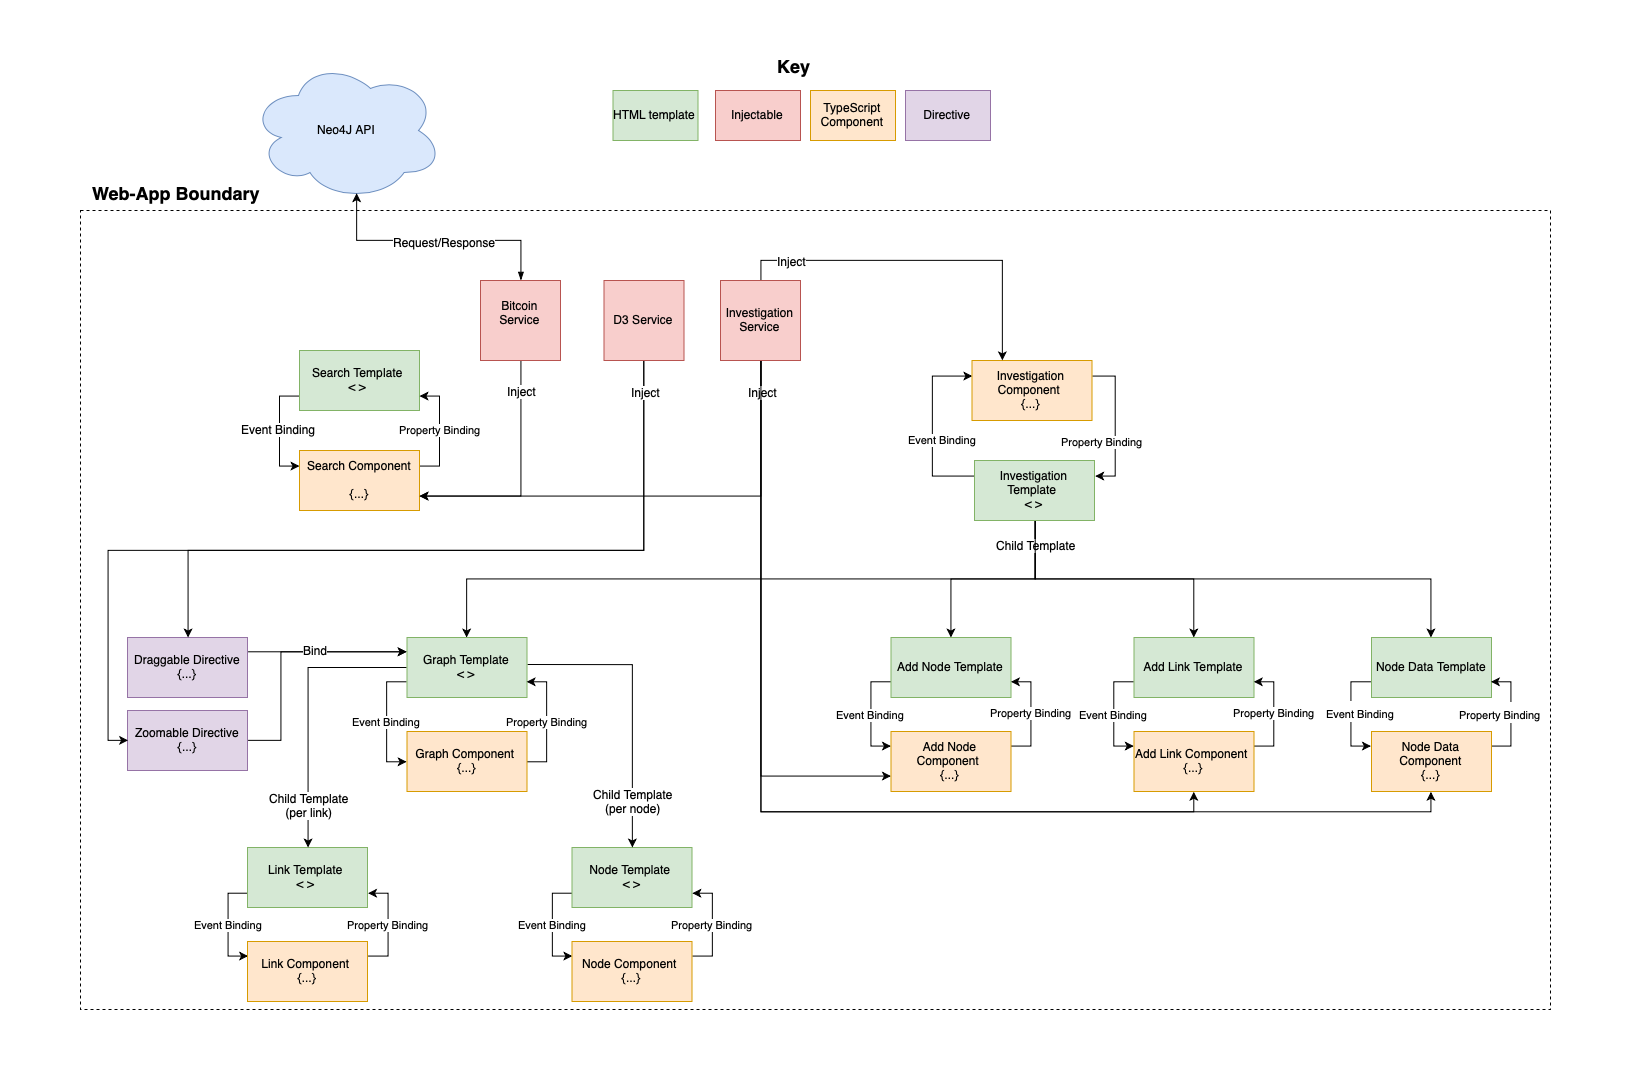
\includegraphics[width = 22cm]{./figures/angular-webapp-architecture}\\[0.5cm]
  \caption{Architecture of the Web Application}
  \label{fig:webapp-architecture}
\end{sidewaysfigure}

\subsection{Search By Address}
An investigation can be initiated by searching for a particular bitcoin address. The search form as shown in figure \ref{fig:neo4j-screenshot-search-form}, when submitted, loads the investigation view displaying the address and it's immediate neighbours as nodes in the graph, also detailing the relationship types each link represents, as shown in figure \ref{fig:neo4j-screenshot-basic-address-nodes}. 

\begin{figure}[h!]
  \centering
  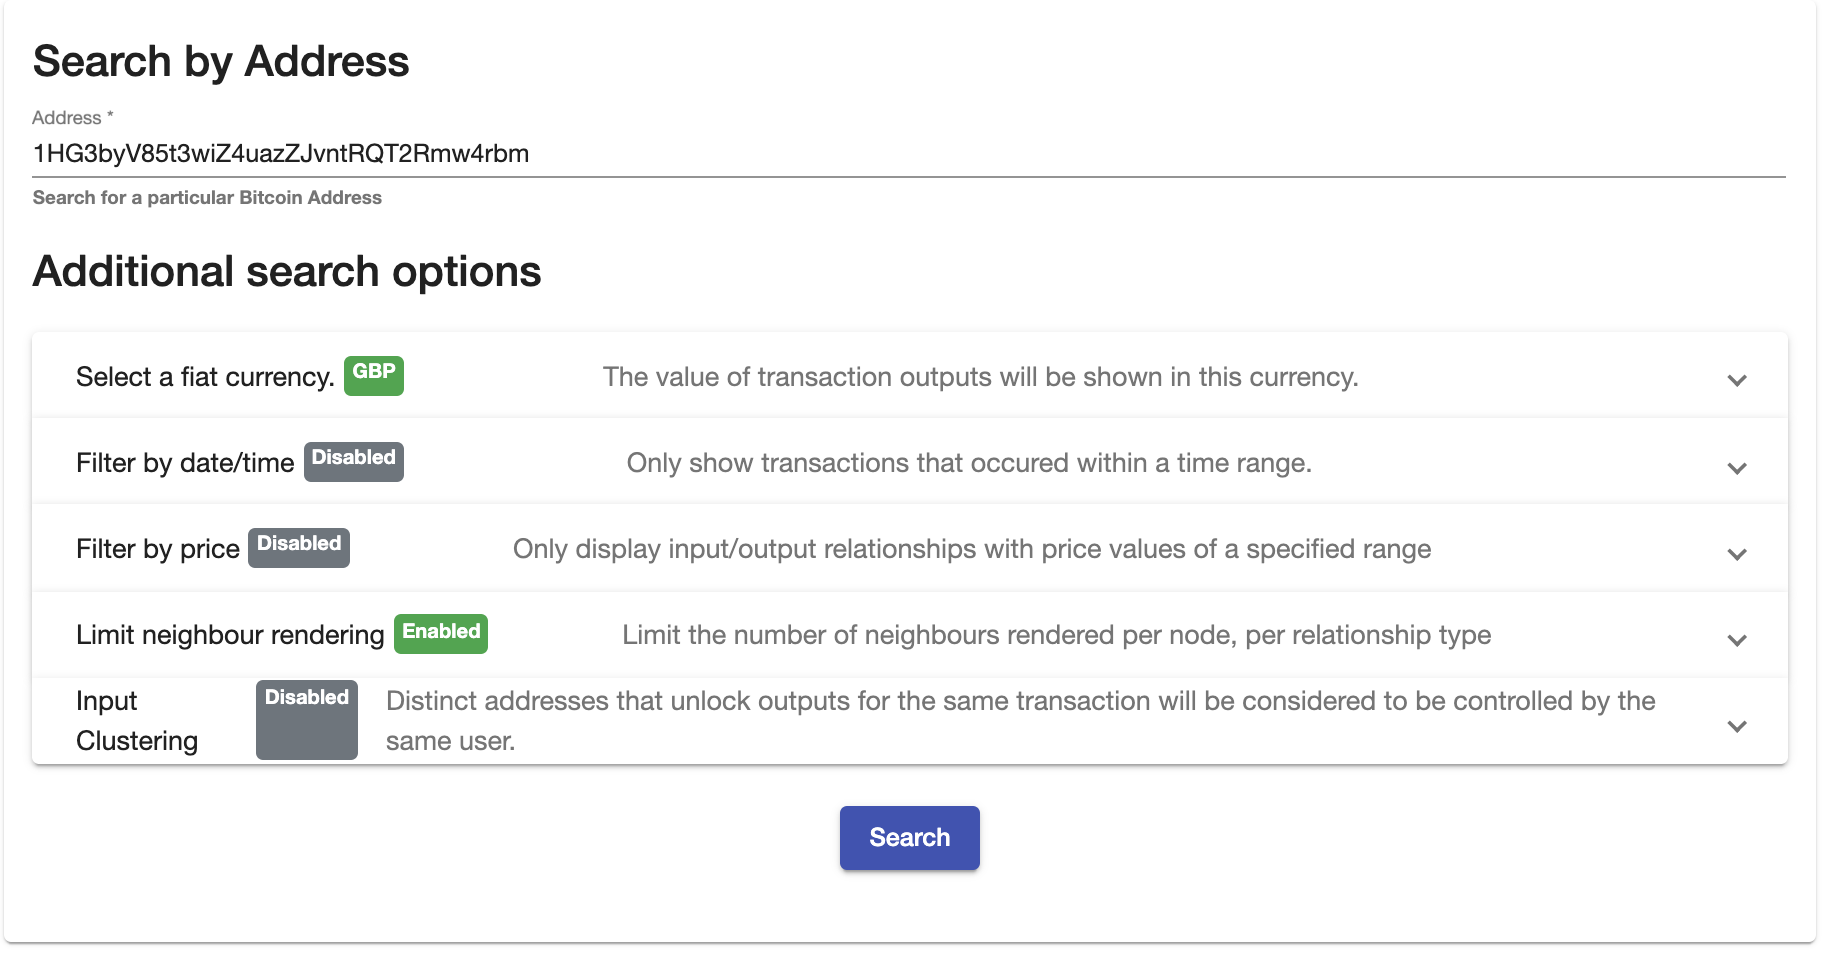
\includegraphics[width = 15cm]{./figures/ui-screenshots/search-address-form}\\[0.5cm]
  \caption{A screenshot of the address search form feature.}
  \label{fig:neo4j-screenshot-search-form}
\end{figure}

\begin{figure}[h!]
  \centering
  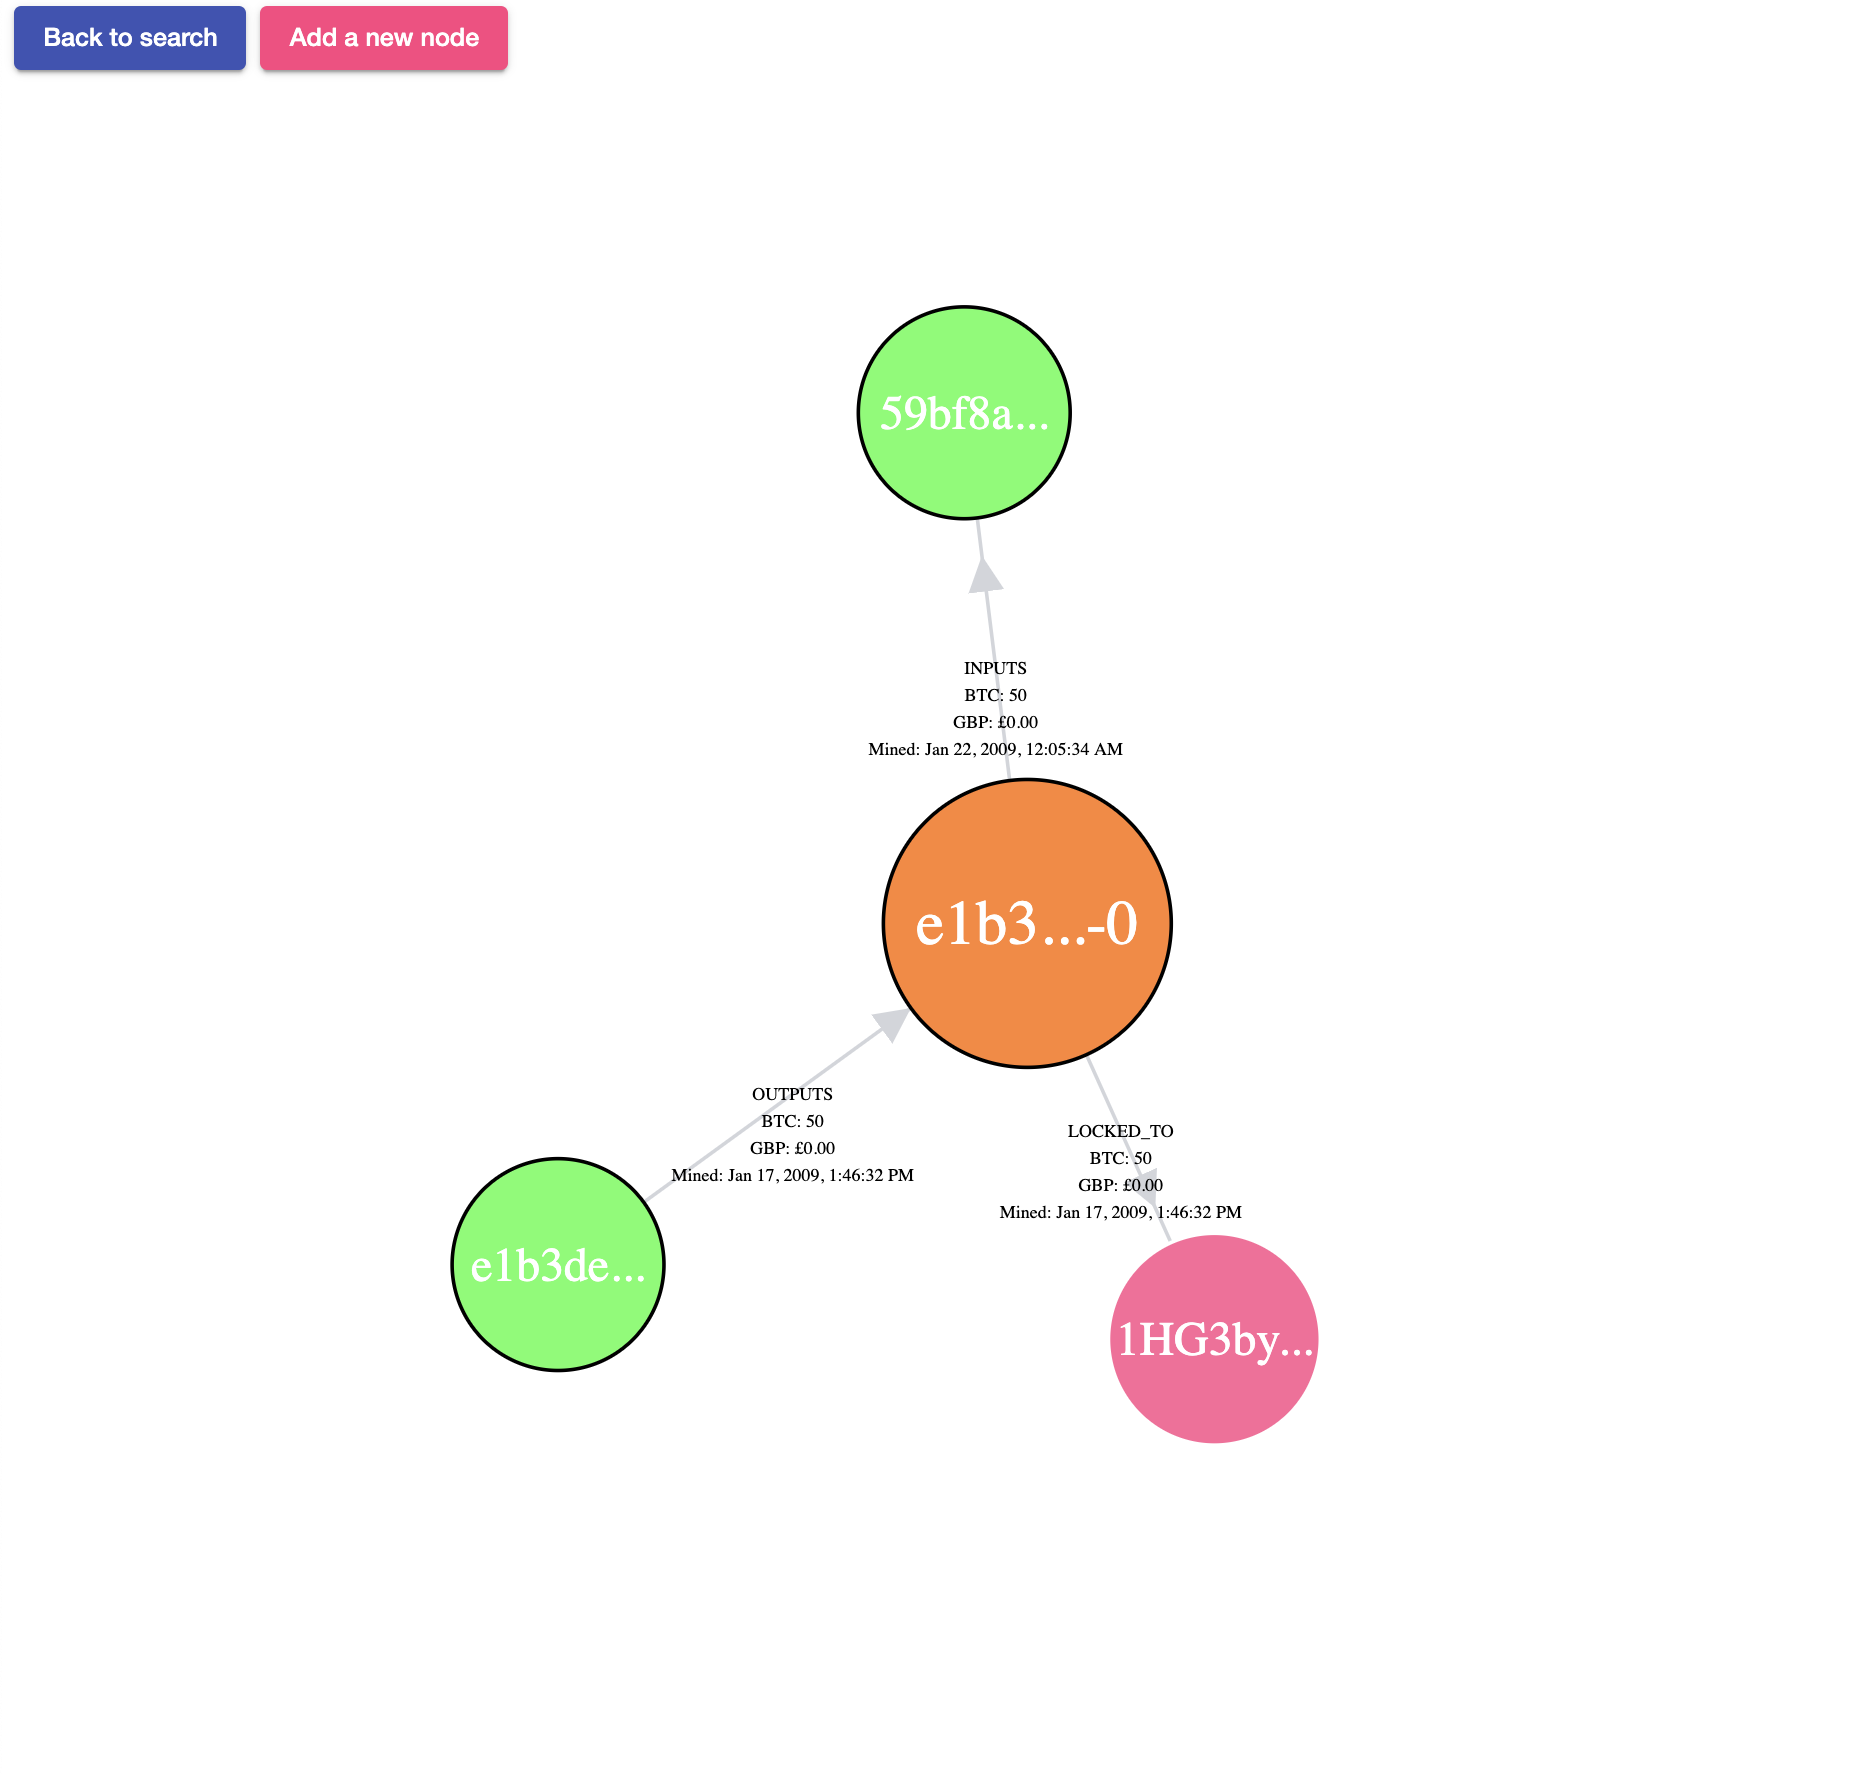
\includegraphics[width = 15cm]{./figures/ui-screenshots/graph-basic}\\[0.5cm] 
  \caption{A screenshot of the search result produced by the search shown in figure \ref{fig:neo4j-screenshot-search-form}}
  \label{fig:neo4j-screenshot-basic-address-nodes}
\end{figure}

\subsection{Node information on hover}
Information associated with each type of node is shown on hover. For example, hovering over a block will provide the time it was mined, its hash and the historical exchange rates at the time of mining (see fig \ref{fig:block-info-on-hover}). The node being hovered over will expand in size to indicate which node the information is being displayed for. There is also an option to dismiss the information box using the cross symbol in the top right corner. 
\\\\
Additionally, clicking on each field in the node information box automatically copys that data to the users clipboard. This further improves the user experience as there exists less steps to copying data (such as long ID's or hashes) for further investigation. The data copied will also be copied without the extraneous surrounding data such as labels, currency symbols or data formatting (specifically, selecting dates will copy the epoch time in milliseconds to the clipboard). 

\begin{figure}[h!]
  \centering
  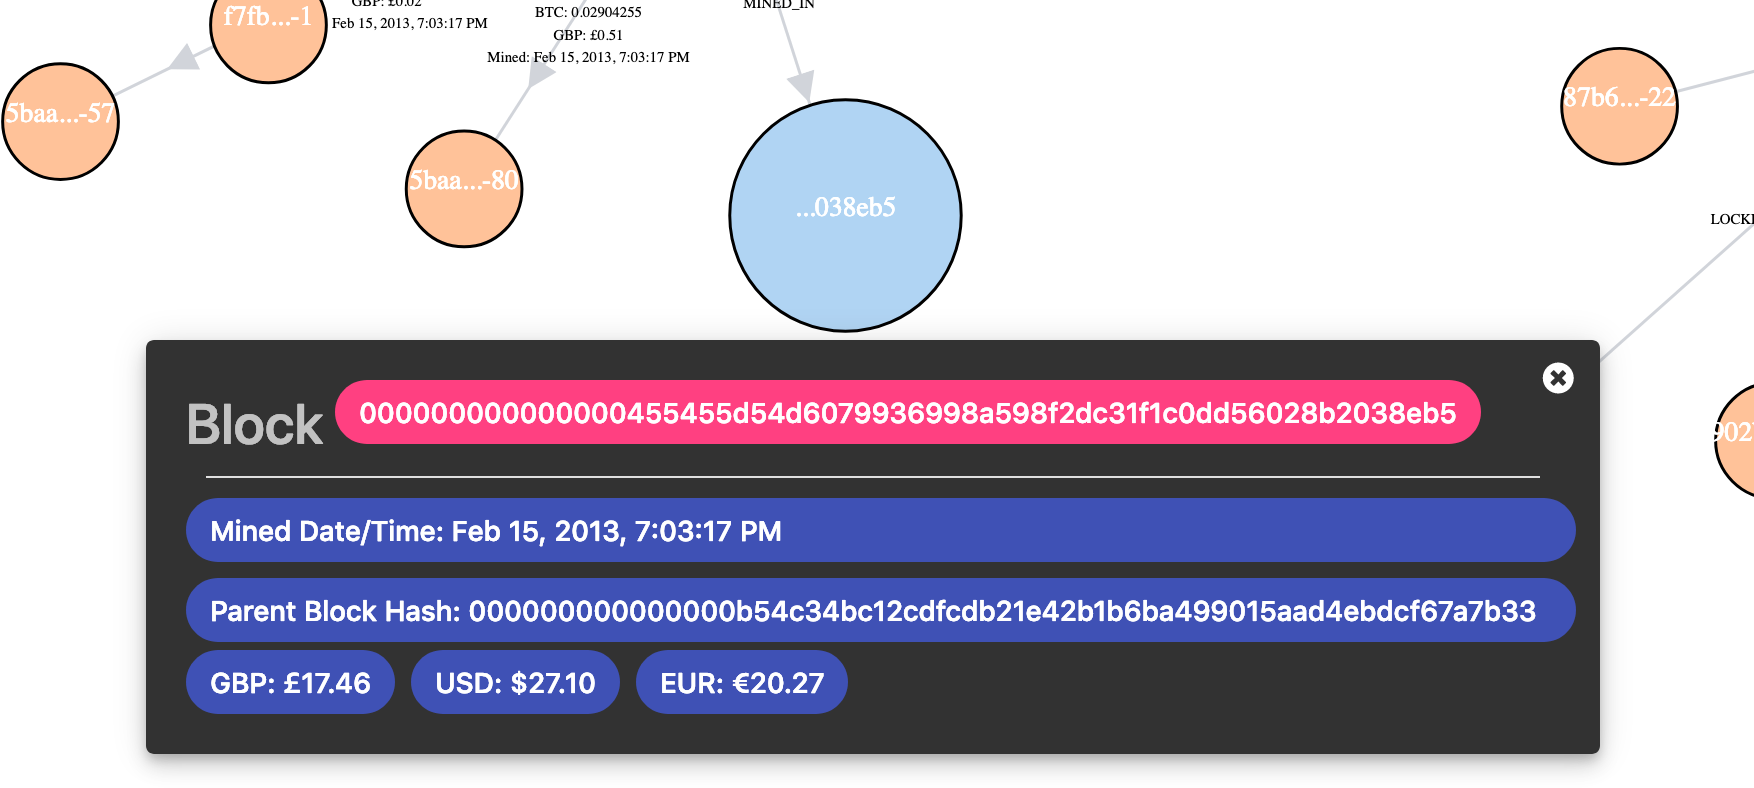
\includegraphics[width = 15cm]{./figures/ui-screenshots/block-info}\\[0.5cm] 
  \caption{A screenshot of block information being displayed when hovering over a block node}
  \label{fig:block-info-on-hover}
\end{figure}

\subsection{Link Data}
A primary use of the investigation tool will be to investigate the flow of funds; it is therefore important to make this information visible and digestible. Therefore, each link representing a flow of funds (between \texttt{OUTPUT} and \texttt{TRANSACTION} nodes) displays the value of the funds in BTC and whichever fiat currency the user selects as their preference when searching (GBP, EUR, USD). The link data also provides a timestamp representing the time the transaction was included in the blockchain; this provides context to the value of the output respective to their fiat currencies. 
\\\\
The screenshot shown in figure \ref{fig:link-data} exemplifies the importance of a fiat currency conversion: the same unit of 0.5 BTC is output by transaction \texttt{432f18...} as is input into transaction \texttt{96455e...}, however their equivalent fiat value in USD is dramatically different at $\$1,688$ when the output is produced and $\$2,102$ when the output is spent. The timestamp will also provide context around the timeline of this transfer of funds, in addition to possibly explaining differences in fiat currencie exchange rates.

\begin{figure}[h!]
  \centering
  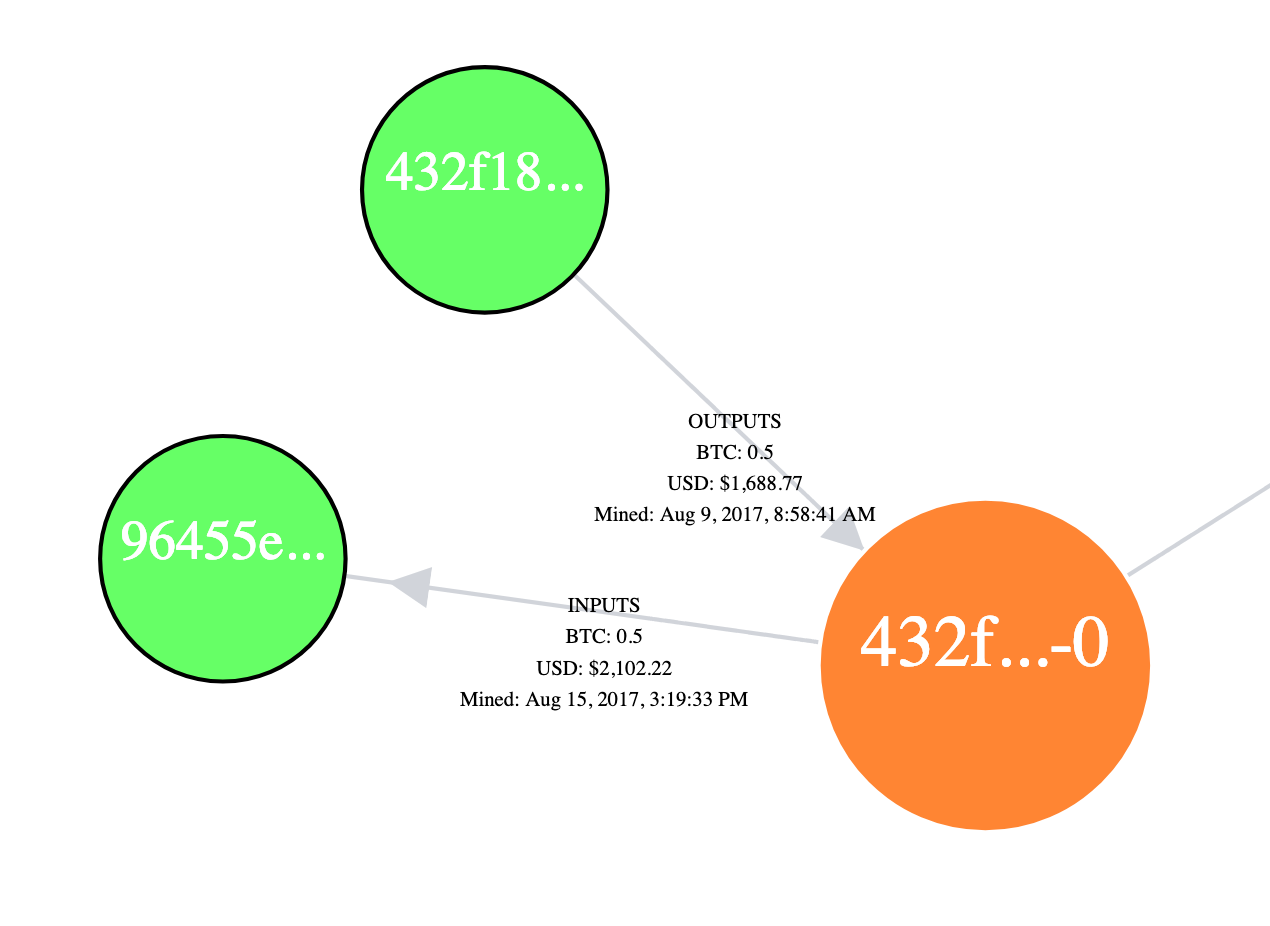
\includegraphics[width = 15cm]{./figures/ui-screenshots/link-data}\\[0.5cm] 
  \caption{A screenshot link data between two transaction nodes (green) and an output node. 
  Transactions IDs are: \texttt{432f18aa46626934c45805046f9c9791fb60bd41da1eb951b47f73bb3b8c7484},\\\texttt{96455e8b6a877f273d14aa13ecb1971577c0d17716b7028c9809c7ca3e1f6e3c}}
  \label{fig:link-data}
\end{figure}

\subsection{Traverse the Graph}
Double clicking on a node initiates a request to load that nodes immediate neighbours. Once the request receives a response, the nodes neighbours are added to the existing graph as new nodes and the necessary links are created. Each new node can then also be double clicked and the process will recurse. 
\\\\
Sometimes the time between initiating a request and receiving a response isn't near instantaneous, perhaps due to demand on the database or a greater response size. Therefore, to feedback to the user that a request has been initiated, to prevent them trying to issue multiple requests or thinking that a node has no neighbours, a node will pulse in size while a request is pending. 
\\\\
Additionally, in an investigation view with many nodes, it may not be clear which nodes already have had their neighbouring nodes requested (those without neighbours, for instance). Therefore, nodes will have a thick black border until their nodes have been expanded (see both green transaction nodes in fig \ref{fig:link-data} and will have their border removed once expanded (see the orange output node in fig \ref{fig:link-data}).

\subsection{Link Dependant Colour and Size of nodes}
To indicate the differences in a nodes connectivity among the many other nodes in the graph, a nodes colour and size adjusts based on the number of links it has outgoing and incident on it. The rate at which a nodes colour and size changes is normalised by the total number of links in the graph. A node with 30\% of the links in a graph of 10 links should have the same size/colour as a node with 30\% of the links in a graph with 100 links. This feature helps with visualising potentially more important nodes in a graph, and also assists with visual arrangement, by creating a greater circumference to place neighbouring nodes around a node with many links. 
\\\\
An example of this can be seen in figure \ref{fig:address-nodes-colour-size-change} where an address \texttt{1HJtS7...} has more links than another address \texttt{1HeYaB...} and therefore has a higher colour density and larger radius. The figure also exemplifies this for output node \texttt{b777...0} which has more links than the other output nodes, and is therefore slightly larger and of a higher density colour.

\begin{figure}[h!]
  \centering
  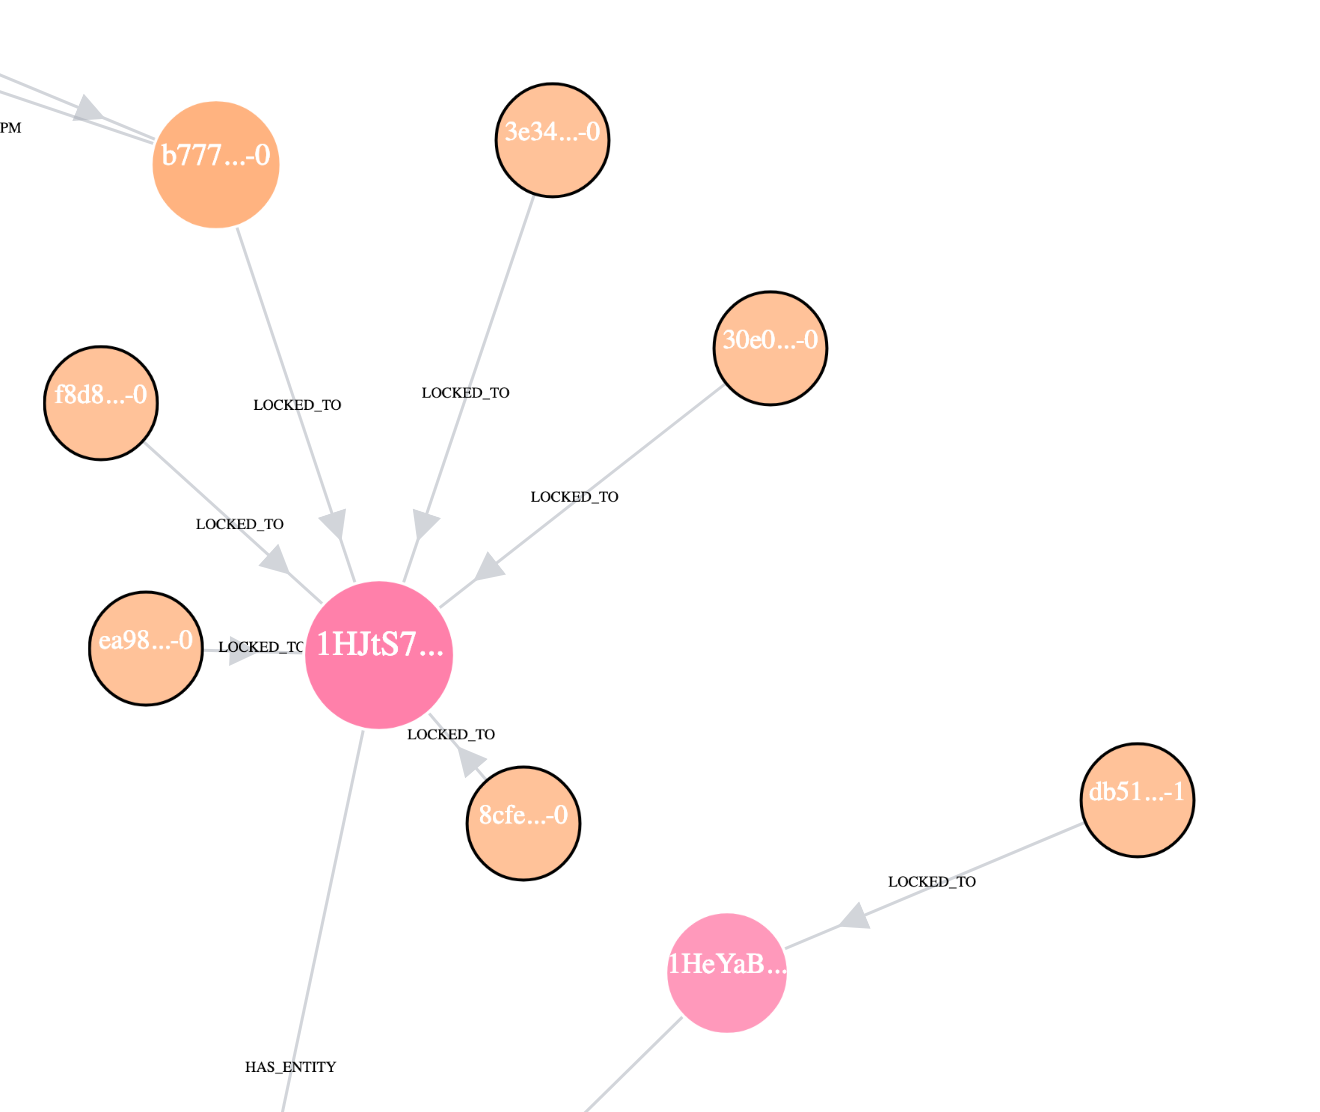
\includegraphics[width = 10cm]{./figures/ui-screenshots/link-dependant-size-colour}\\[0.5cm] 
  \caption{A screenshot of two address nodes, with a varying number of links each.
  Address IDs are: \texttt{1HJtS7wLaqdZRf1Cd4FfJDEWL17VJVDcm2},\\\texttt{1HeYaB7gntUXQBtLaeJmqWzAdFf2PWMEfZ}}
  \label{fig:address-nodes-colour-size-change}
\end{figure}

\subsection{Add nodes with complementary}

\subsection{Filter Date/Time}

\subsection{Filter by value, several currencies}

\subsection{Enable Multi-input clustering view}

\subsection{Configure how many nodes to display}

\subsection{User Input Validation}

\subsection{Loading feedback states}

\subsection{Limiting nodes}

